La figure \ref{fig:chaineacquisition} reprend la chaîne d'acquisition finale\footnote{Une version plus grande et en couleur de la chaîne est disponible dans l'Annexe \ref{chaineacquiannexe}}. On peut remarquer un ajout qui n'a pas été mentionné : il s'agit du filtre passe-bas entre l'alimentation et la polarisation du microphone et du signal avant amplification. Nous avons remarqué que le bruit du signal était important dans un milieu calme. Le filtre passe-bas permet d'atténuer ce bruit qui est en partie causé par l'alimentation.

\begin{figure}[H]
    \centering
    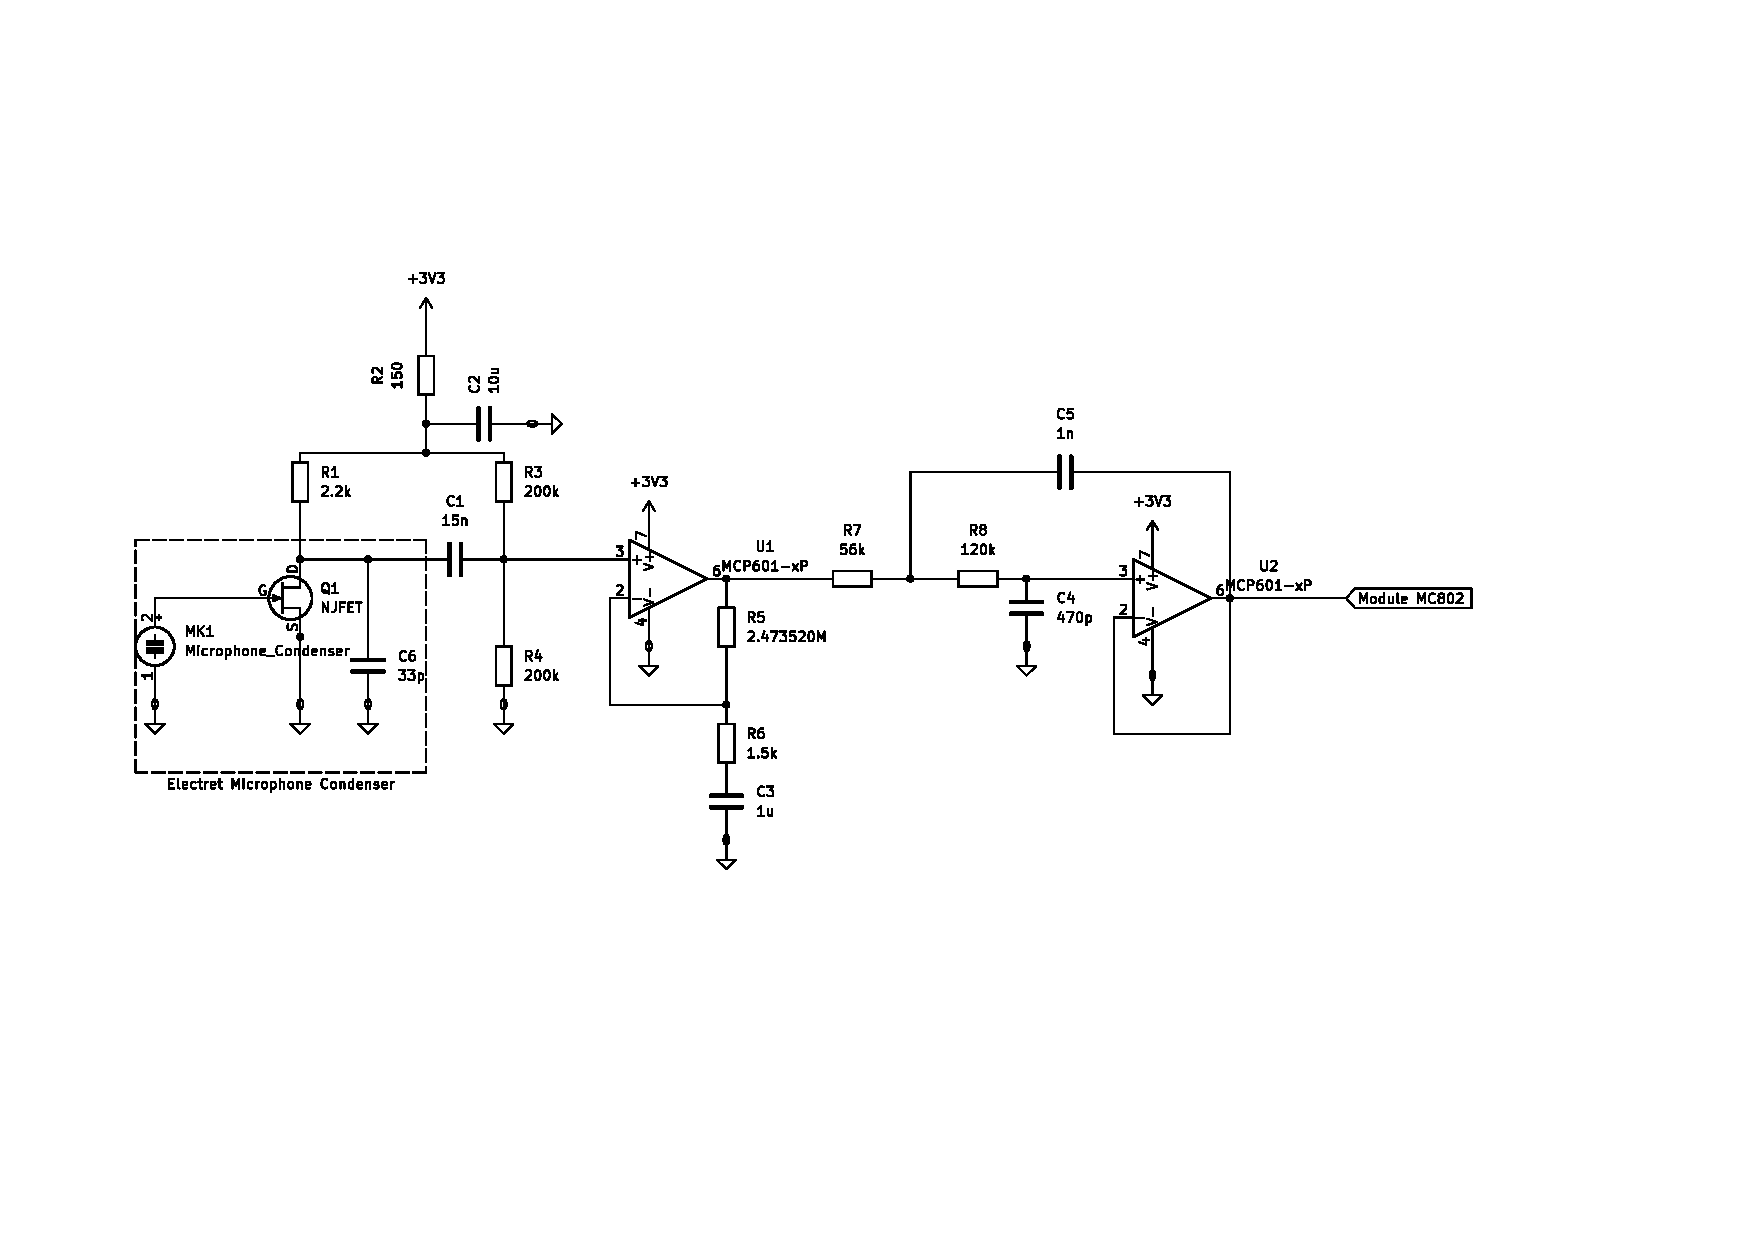
\includegraphics[width=1.2\textwidth]{pdffiles/chainacquiCompacBlack.pdf}
    \caption{Chaîne d'acquisition}
    \label{fig:chaineacquisition}
\end{figure}

\subsubsection{Validation de la chaîne d'acquisition}

Pour clôturer la section sur la chaîne d'acquisition, il faut s'assurer que cette partie du projet fonctionne correctement.
Dans un premier temps, on observe le signal de sortie de la chaîne à l'aide du Picoscope et on s'assure que les points suivants sont respectés :

\begin{itemize}
    \item [$\bullet$] Le signal est centrée en $1.65 \ V$
    \item [$\bullet$] Le signal varie de $0 \ V$ à $3.3 \ V$ pour des fréquences aux alentours de $1000 \ Hz$
    \item [$\bullet$] Le signal est atténué pour des fréquences suffisamment éloignées de $1000 \ Hz$
\end{itemize}

Sur les figures \ref{fig:sortie400}, \ref{fig:sortie900} et \ref{fig:sortie4000} se trouvent le signal après amplification en bleu et le signal de sortie final en rouge pour des signaux sonores de 400 Hz, 900 Hz et 4000 Hz. On remarque que tous les points énoncés précédemment sont respectés

\begin{figure}[H]
    \centering
    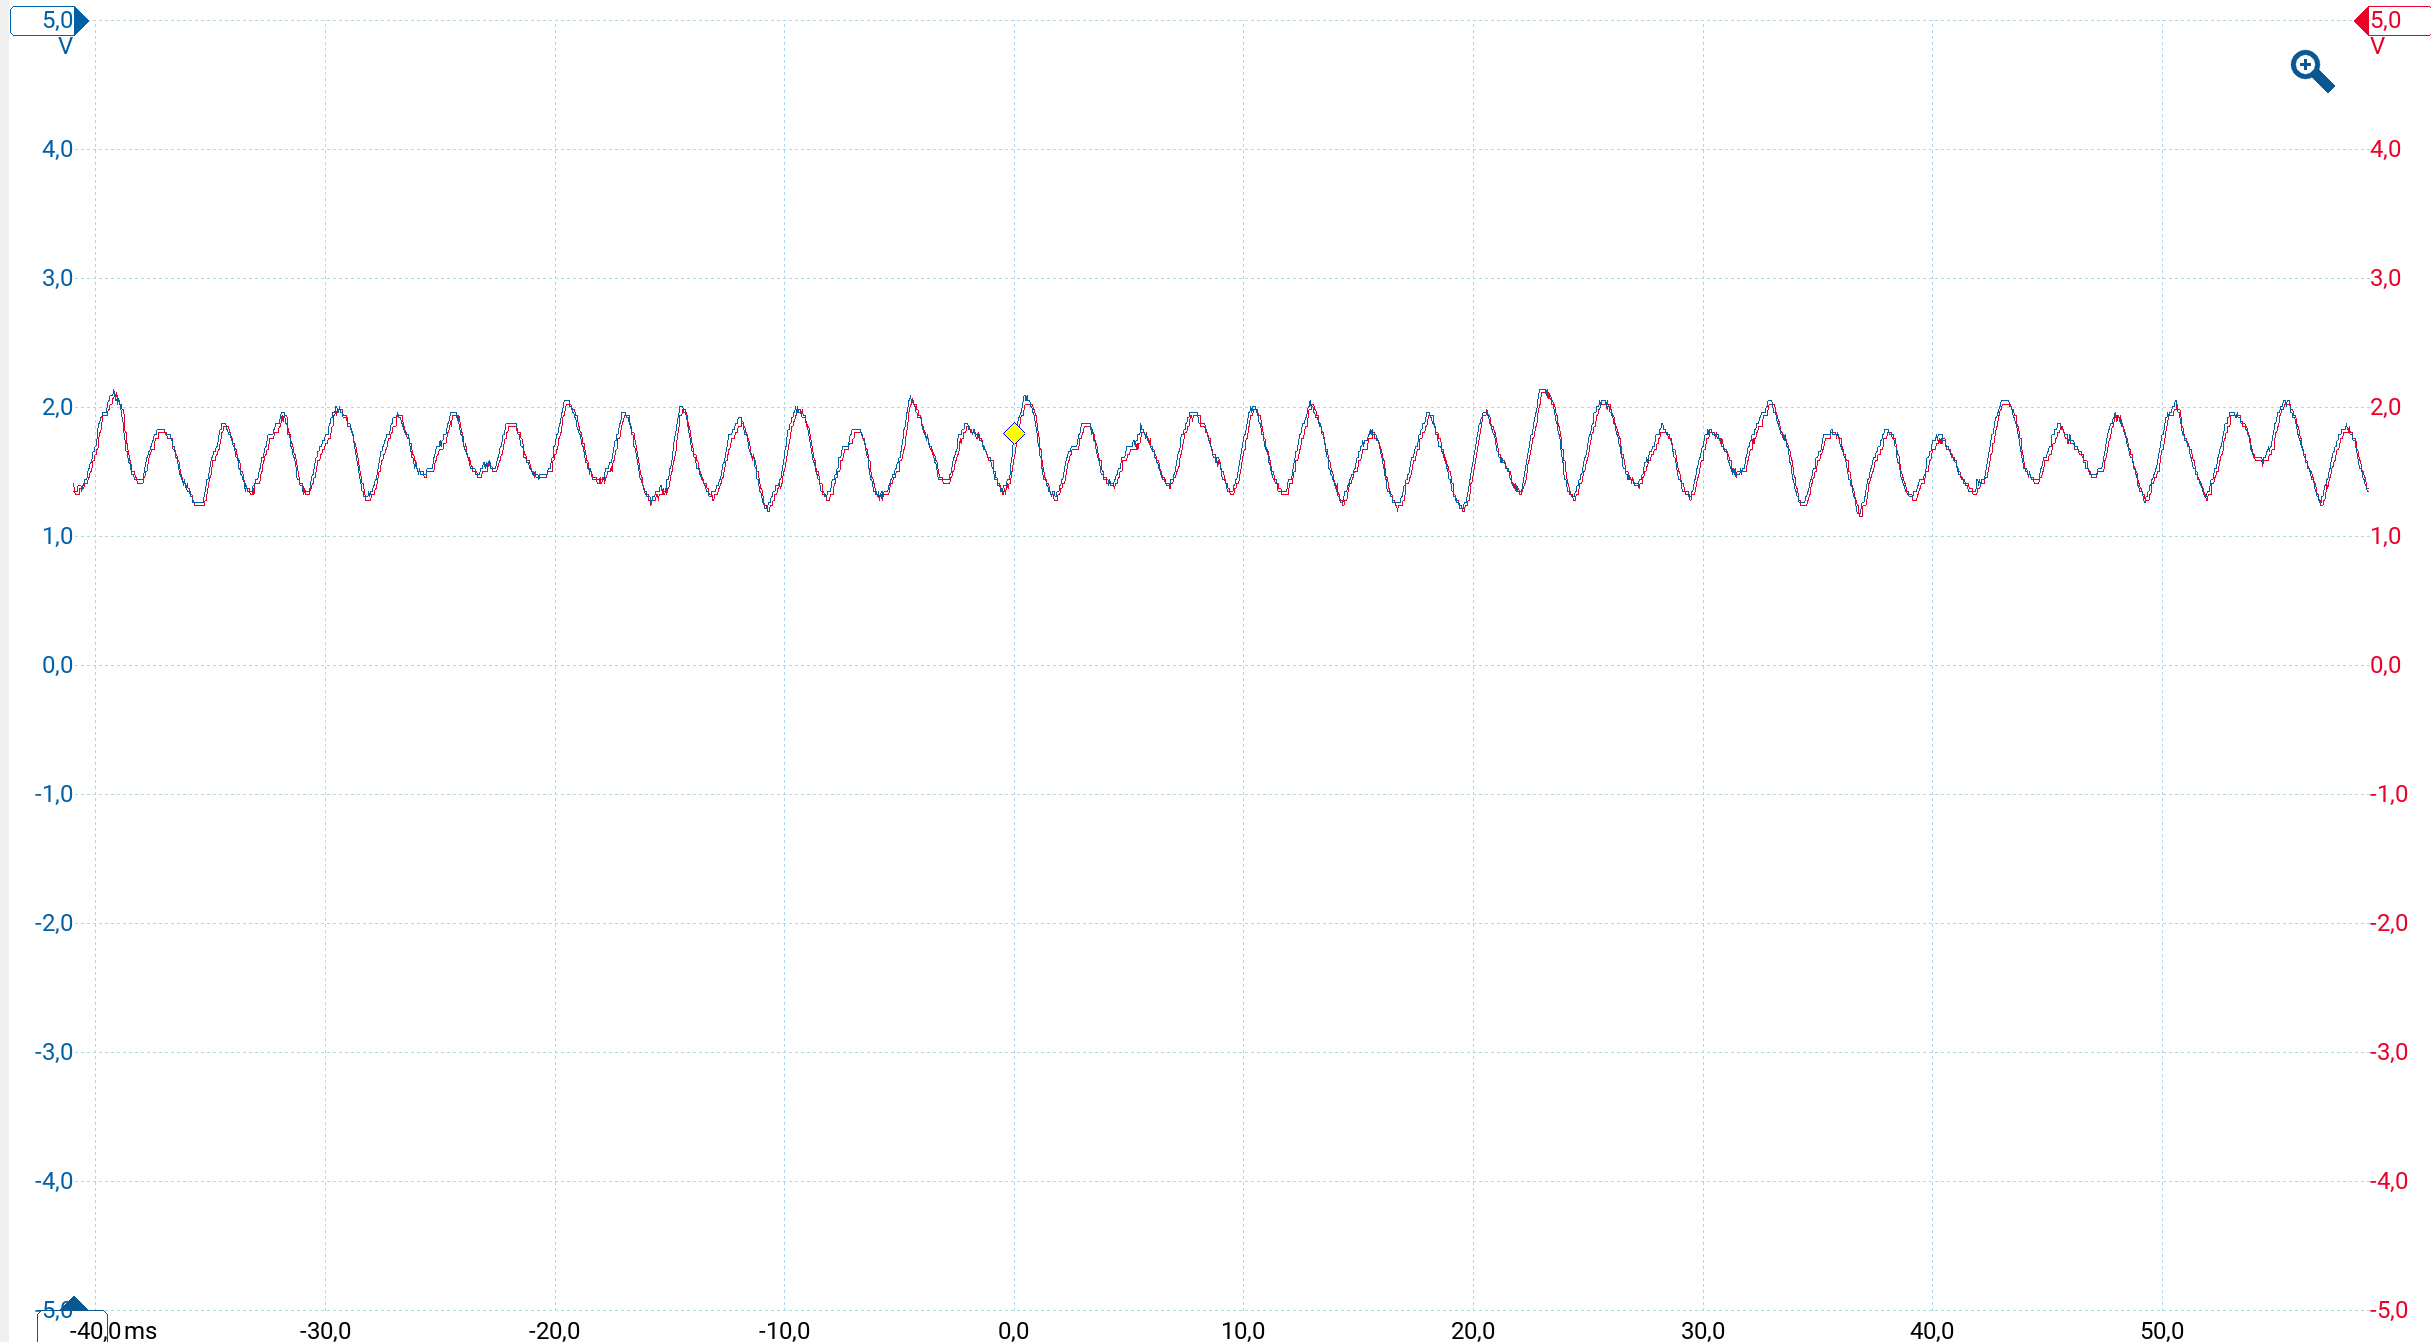
\includegraphics[width=0.6\textwidth]{Pictures/400Hz.png}
    \caption{Signal de sortie de la chaîne pour un signal audio de 400 Hz. Signal après amplification en bleu, signal de sortie final en rouge}
    \label{fig:sortie400}
\end{figure}

\begin{figure}[H]
    \centering
    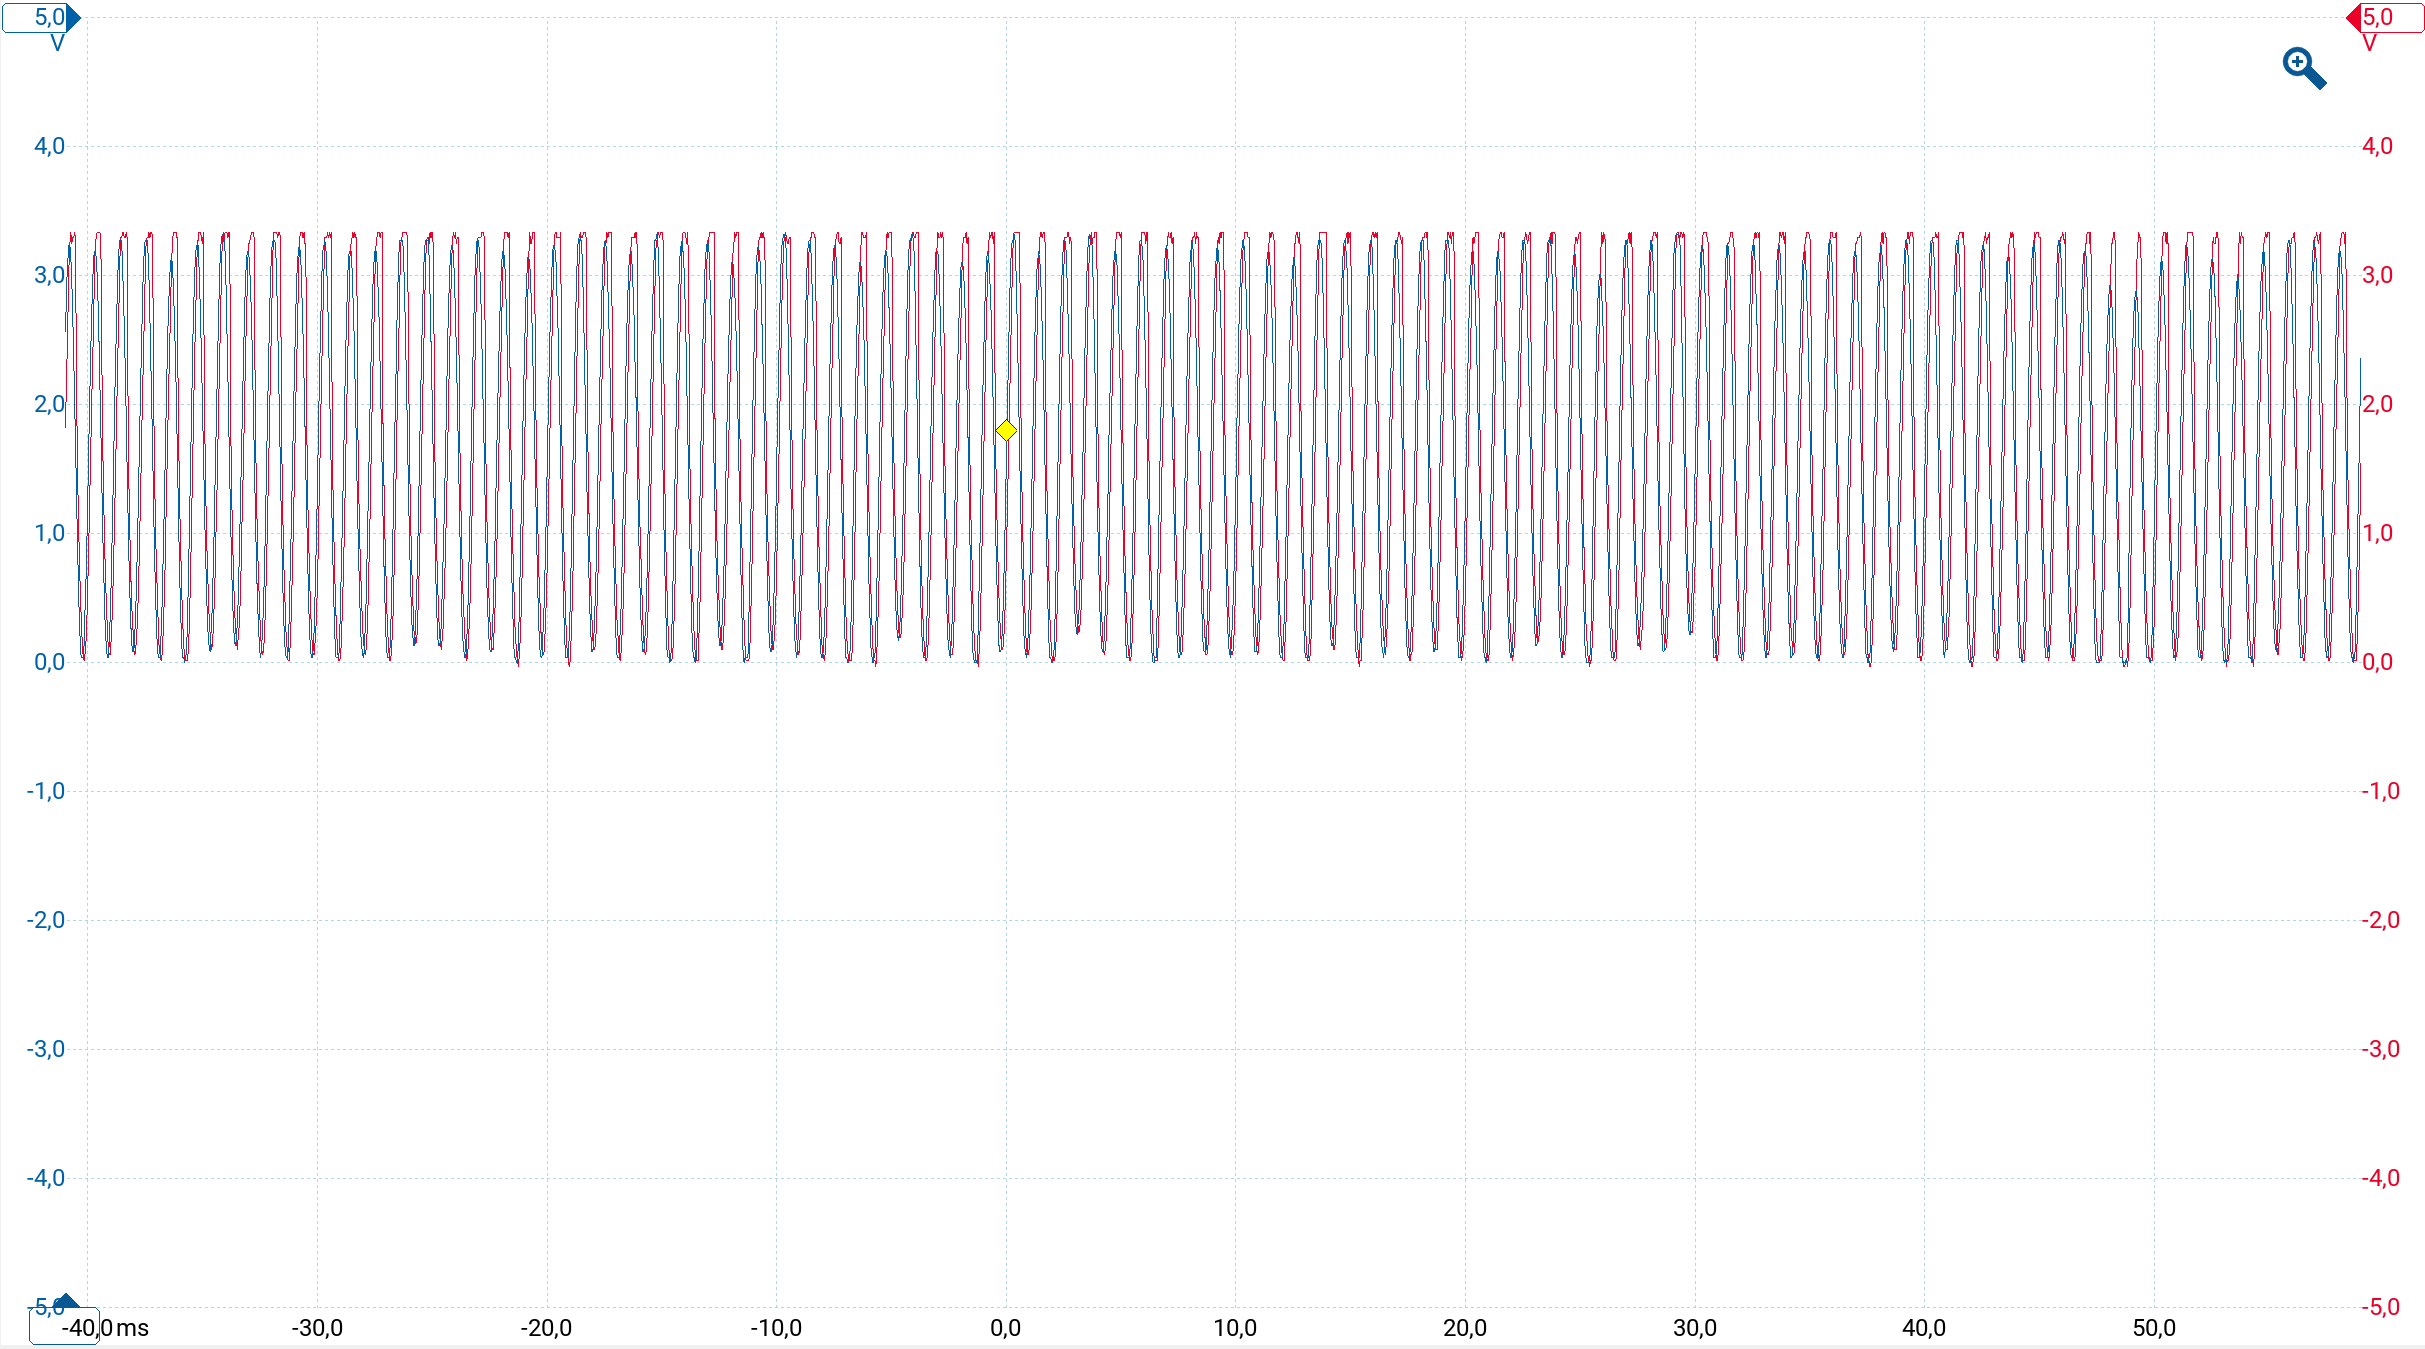
\includegraphics[width=0.6\textwidth]{Pictures/900Hz.png}
    \caption{Signal de sortie de la chaîne pour un signal audio de 900 Hz. Signal après amplification en bleu, signal de sortie final en rouge}
    \label{fig:sortie900}
\end{figure}

\begin{figure}[H]
    \centering
    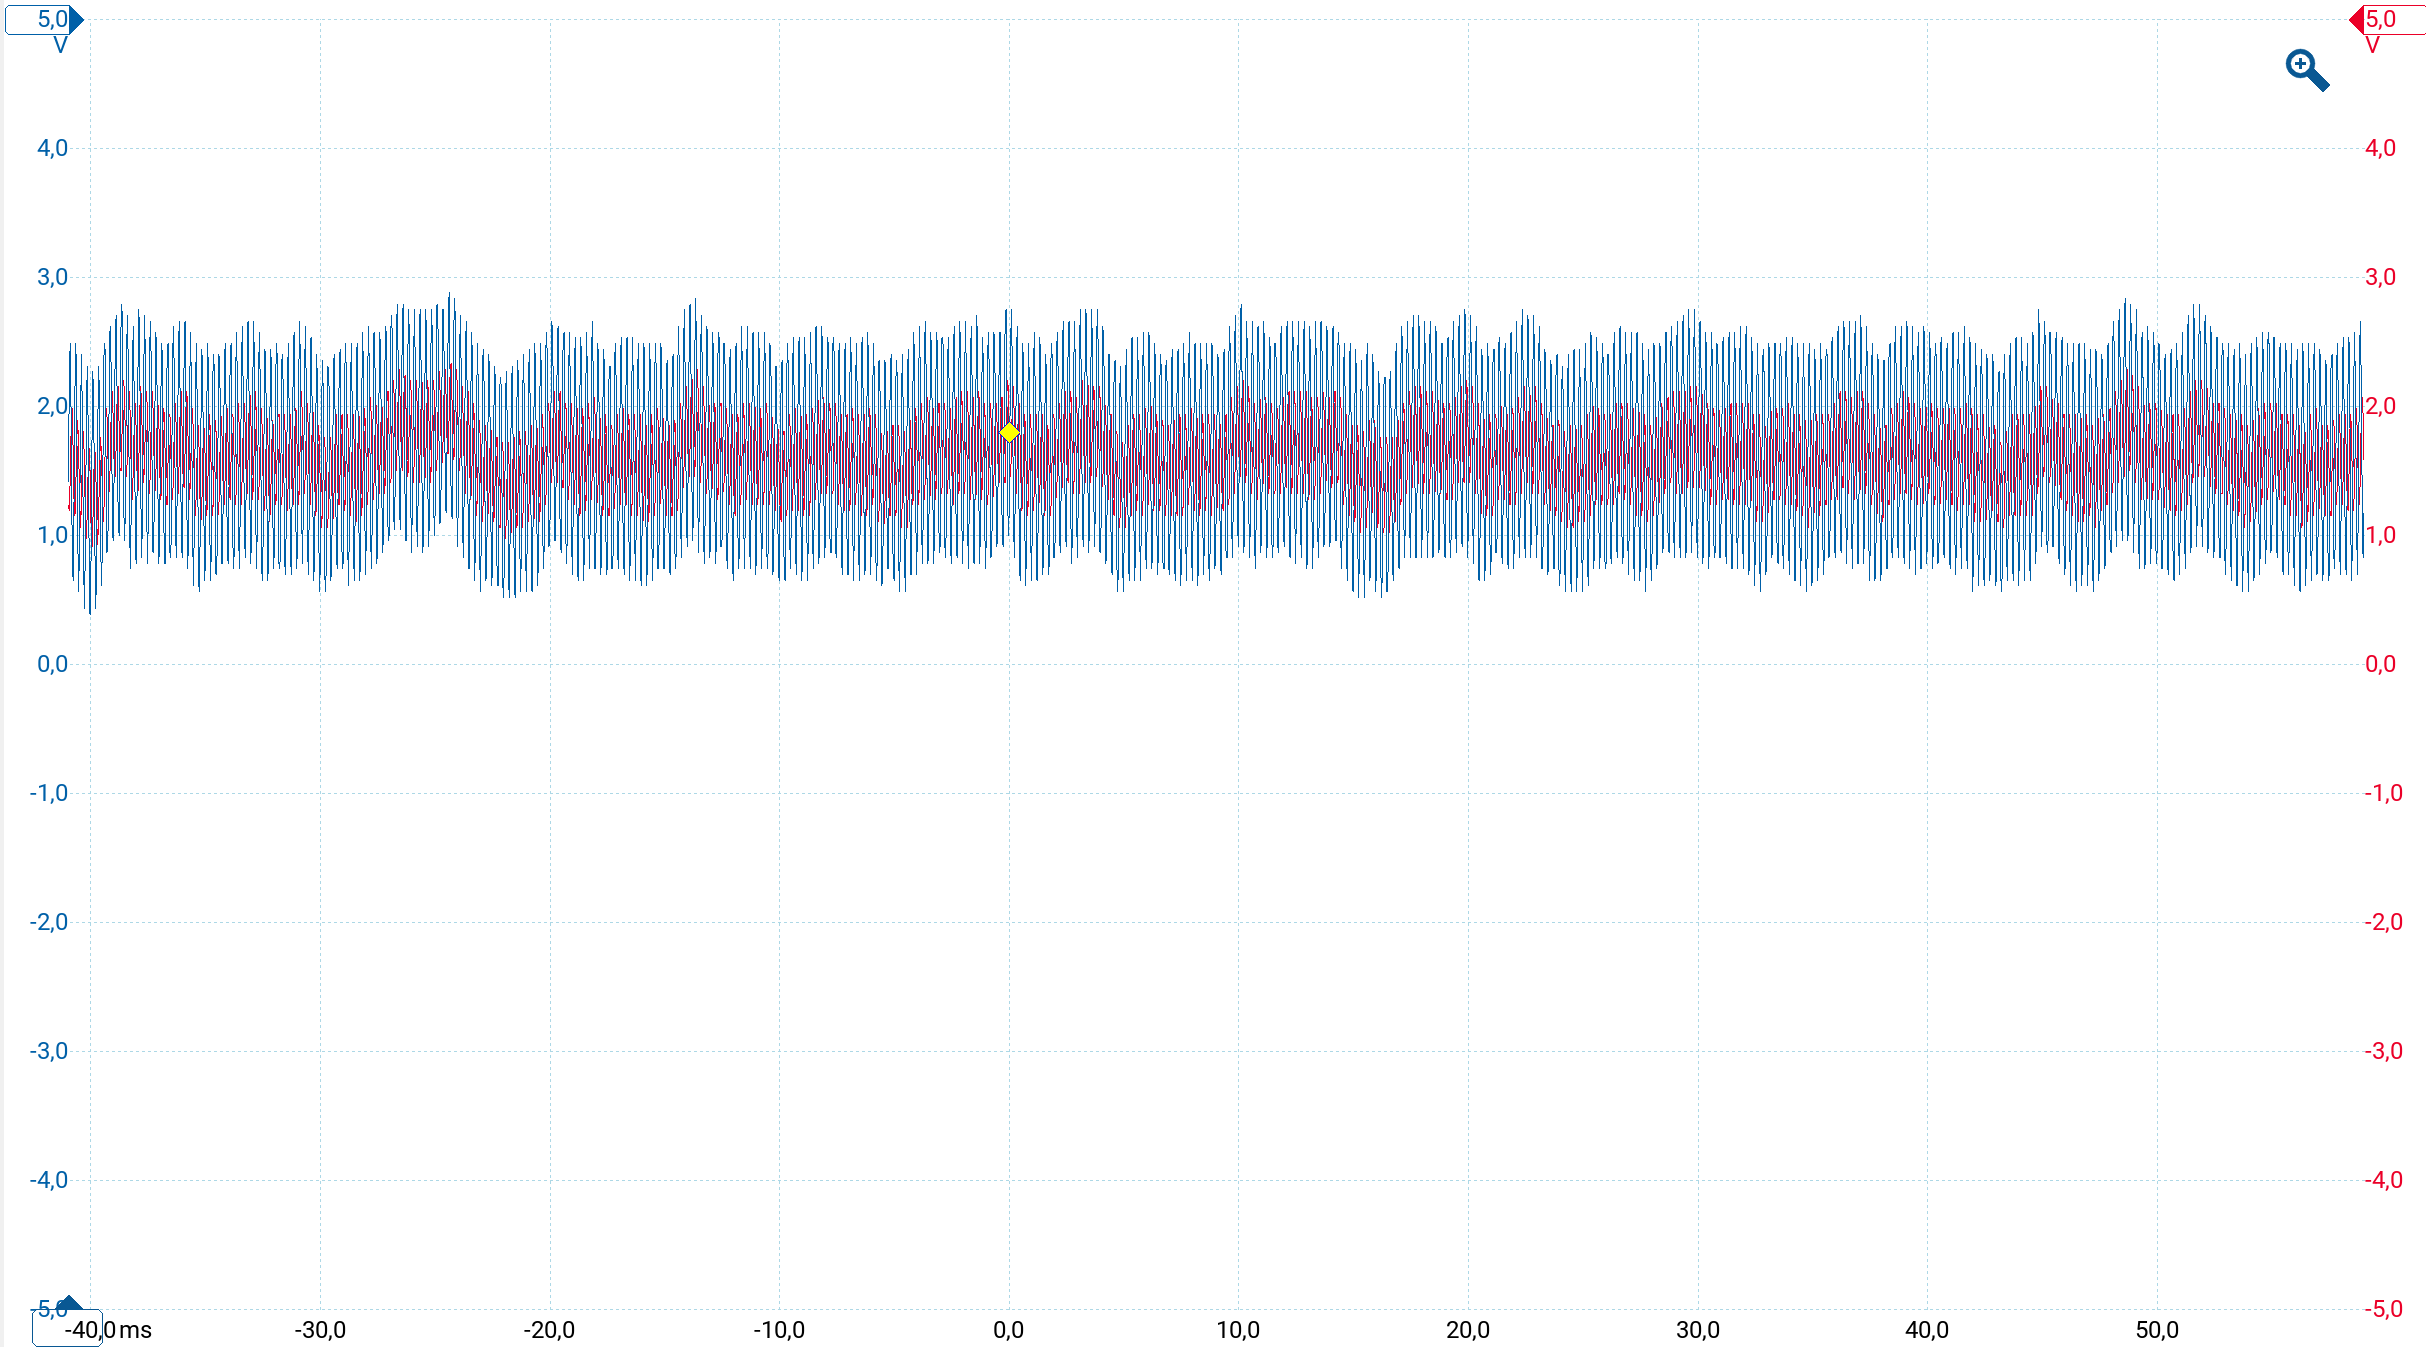
\includegraphics[width=0.6\textwidth]{Pictures/4000Hz.png}
    \caption{Signal de sortie de la chaîne pour un signal audio de 4000 Hz. Signal après amplification en bleu, signal de sortie final en rouge}
    \label{fig:sortie4000}
\end{figure}

Dans un second temps, on doit vérifier que la chaîne fonctionne pour un signal de commande audio. Pour ce faire, on utilise le \textit{canal math} du Picoscope qui affiche la fréquence du signal en fonction temps. Si on observe clairement un changement de fréquence lorsque le signal de commande audio est émis, on peut en conclure que la chaîne fonctionne correctement. La figure \ref{fig:testacqui} montre ce test et on remarque que le signal en blanc qui représente la fréquence au cours du temps varie.

\begin{figure}[H]
    \centering
    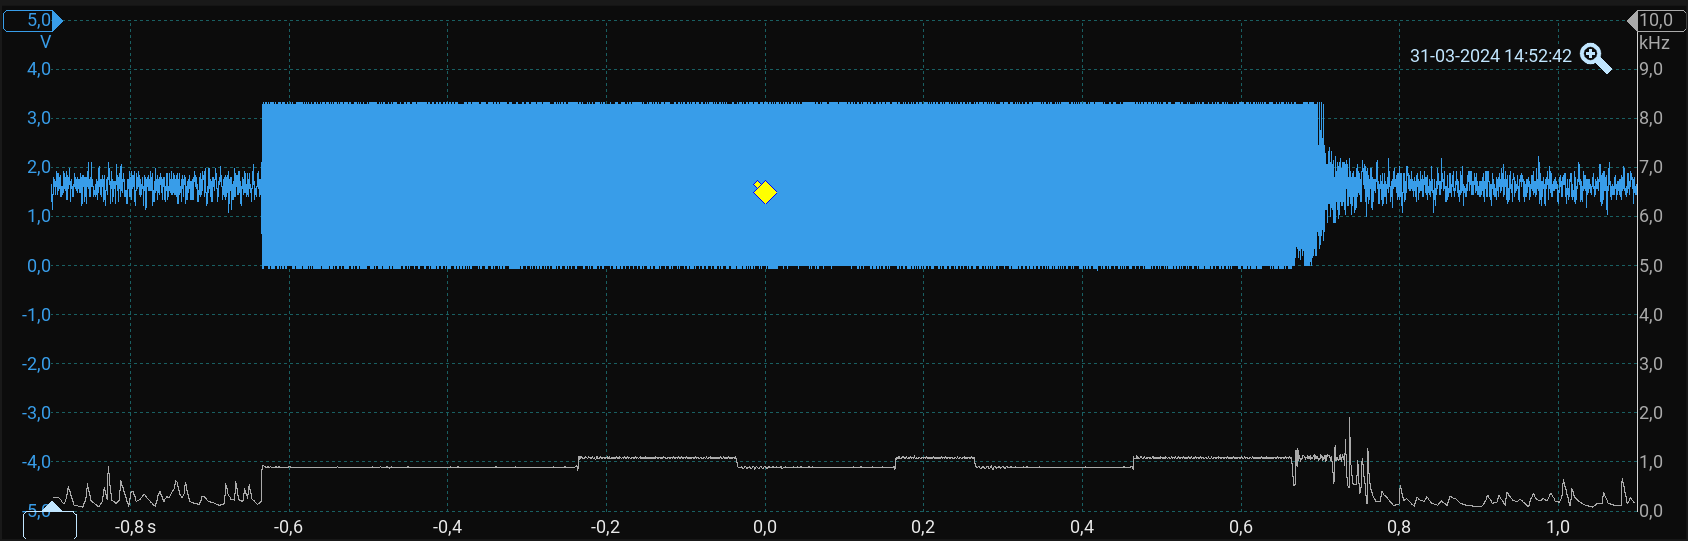
\includegraphics[width=0.8\textwidth]{Pictures/testchaineacqui.png}
    \caption{Signal de sortie de la chaîne et sa fréquence pour une commande audio. Le signal de sortie est en bleu et la fréquence du signal au cours du temps en blanc.}
    \label{fig:testacqui}
\end{figure}

Avec ces deux tests, on peut valider le bloc \textbf{Chaîne d'acquisition} de la partie \textbf{Traitement des signaux audio} du projet. %Cependant, il y a quelques points à adresser avant de continuer.